\chapter{Monte Carlo Samples }\label{section:star_mc}
\ac{MC} samples used to correct data for detector effects were obtained by the embedding \ac{MC} technique~\cite{STAR:tpc}, in which  simulated particles are mixed with the real Zerobias events at the raw data level. Zerobias data events used in the embedding were sampled over the entire data-taking period in order to properly describe the data set used in the analysis.  Two samples of embedding MC were produced:
\begin{enumerate}
	\item Single particle \ac{MC}, in which particles are generated from flat distributions in $\eta$ and $p_\textrm{T}$, in order to have similar statistics in all bins.
	\item The \ac{SaS} model implemented in PYTHIA8 with 4C tune. 
\end{enumerate}
The particles were propagated through the full simulation of the STAR-TPC and RP system detectors using GEANT3~\cite{GEANT:three} and GEANT4~\cite{GEANT:four}, respectively. Obtained information for the simulated particles was embedded into the existing information of the real data. These events were next processed through the~full reconstruction chain. 

It is preferred to get the detector corrections from a~MC, which is dedicated to simulate the~studied  physics process. However, for this purpose, the statistics in the MC should be several times greater than we have in the data for analysis. Since this is not possible with  low efficiency of TPC and TOF, the basic method of corrections used in the analysis is a~method of factorization of global efficiency into the product of single-particle efficiencies. In this way, statistically precise multidimensional corrections on TPC and TOF are obtained from the single particle MC.

Additionally, several pure MC samples were generated. The simulated particles were propagated through full simulation and reconstruction chain but were  not embedded  into Zerobias events.   
Systematic effect related to hadronization of the diffractive system was determined by using an~alternative hadronization model implemented in HERWIG. The~comparison to the corrected data distribution was done for PYTHIA 8 4C (\ac{SaS}) and HERWIG, in addition all results were compared to the EPOS and alternative PYTHIA 8 model  \ac{MBR}  with A2 tune. EPOS predicts very large contribution of forward 
protons, which originate from non-diffractive events and are well separated in rapidity from other final state particles. This is the result of low mass excitation of the proton remnant ($<1$ GeV) leading to hadronization of the beam remnant back to the proton. Therefore for the comparison with uncorrected data EPOS predictions were separated in two classes: diffractive (EPOS-SD) modelled by Pomeron exchange and non-diffractive modelled  by low mass excitation of the proton remnant (EPOS-SD$^\prime$). In all PYTHIA~8 models, diffractive cross-sections are scaled by the~fudge factors, which were introduced in order to describe the~full phase space~\cite{Sjostrand:2006za,MBR:intro}. As a result, diffractive cross sections are arbitrary suppressed at 
relatively large values of $\xi$ ($>$0.05). This arbitrary suppression significantly changes predicted distribution of $\xi$ and fractions of different processes in our fiducial phase space. Therefore data was also compared with expectations obtained without suppression of the~diffractive cross sections (MBR-tuned).

Figure~\ref{fig:STARtrueMC} shows $\xi$ and $|t|$ distributions generated with  EPOS (SD and SD$^\prime$) and PYTHIA~8 SD (MBR and MBR-tuned). There are differences among models in both the~low and high $\xi$ regions. In the~STAR acceptance region, there is a~significant contribution of SD$^\prime$ in EPOS, while SD contribution is suppressed. In addition, the $t$-slope is  very different for EPOS-SD and SD$^\prime$ compared to PYTHIA~8 predictions. The~PYTHIA~8 (MBR-tuned) expectations, as opposed to the~MBR model,  lead
to the~larger cross-sections in the high-mass regions.
 
\begin{figure}[h!]
	\centering
	\includegraphics[width=0.49\textwidth, page=14]{chapters/dataSampleSTAR/img/true.pdf}
	\includegraphics[width=0.49\textwidth, page=13]{chapters/dataSampleSTAR/img/true.pdf}
	\caption{(left) $\xi$ and  (right) $|t|$ distributions for various MC generators at $\sqrt{s} = 200$~GeV.}
	\label{fig:STARtrueMC}
\end{figure}